\section{Architecture:}
Une instance Cassandra est une collection de nœuds indépendants qui sont configurés ensemble pour former un cluster.

Dans un cluster, tous les nœuds sont égaux, ce qui signifie qu'il n'y a pas de nœud maître ou un processus centralisant leur gestion.

En fait, Cassandra utilise un protocole appelé Gossip afin de découvrir la localisation et les informations sur l'état des autres nœuds du cluster. Le protocole Gossip est un protocole de communication de type "peer-to-peer" dans lequel les nœuds échangent périodiquement des informations sur leur état mais également sur ce qu'ils savent des autres nœuds.

Pour être plus précis, le processus s'exécute toutes les secondes afin d'échanger les messages avec au plus trois autres nœuds du cluster. De plus, une version est associée à ces messages afin de permettre d'écraser les informations plus anciennes.

Ainsi, quand un nœud démarre, il regarde dans son fichier de configuration les points de ralliement (SEED) qui devront au moins être contactés une fois.

\begin{figure}[h]
	\centering
    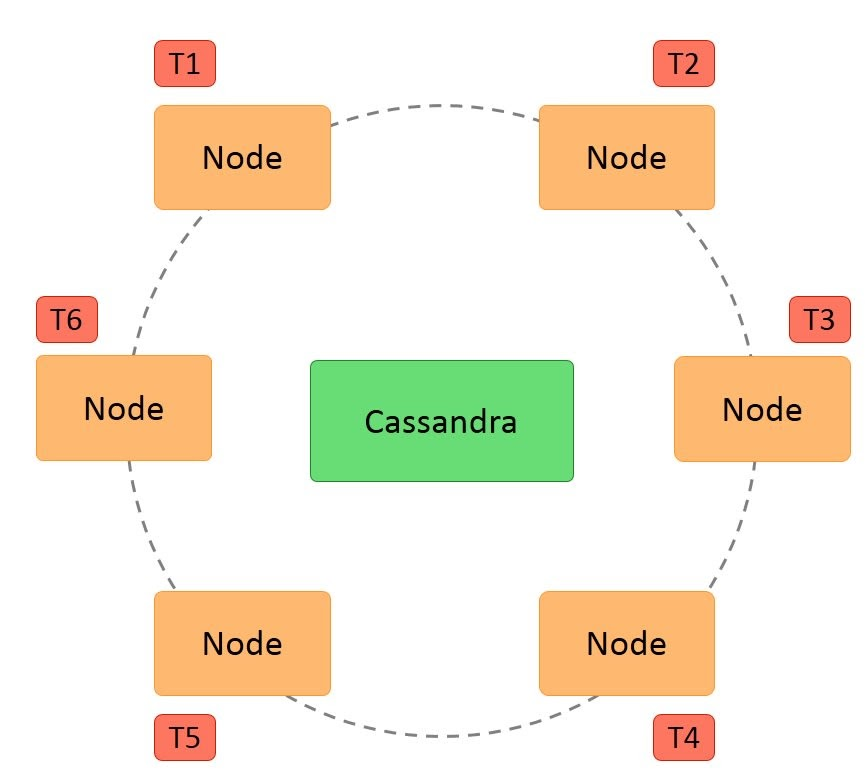
\includegraphics[scale=0.2]{img/part1/5.2}
    \caption{Architecture CASSANDRA}
\end{figure}

Cependant, afin d'éviter un partitionnement, tous les nœuds du cluster doivent disposer de la même liste de nœuds dans leur fichier de configuration.

La détection des échecs est une méthode pour déterminer localement si un autre nœud est accessible ou pas. En outre, les informations récoltées par ce mécanisme permettent à Cassandra d'éviter d'émettre des requêtes aux nœuds qui ne sont plus accessibles.

En fait, ce mécanisme fonctionne sur le principe de heartbeat soit de manière directe (en récoltant les informations directement des nœuds) soit de manière indirecte (en récoltant les informations par l'intermédiaire de la connaissance des autres nœuds).

Lorsqu'un nœud est déclaré comme inaccessible, les autres nœuds stockent les messages susceptibles d'avoir été manqués par ce nœud. Cependant, il peut arriver qu'entre le moment où le nœud devient inaccessible et le moment où sa perte est détectée, un laps de temps s'écoule et qu'ainsi, les réplicas ne soient pas conservés. En outre, si le nœud vient à être indisponible pendant une période trop importante (par défaut, une heure), alors les messages ne sont plus stockés. C'est pour cette raison qu'il est conseillé d'exécuter régulièrement l'outil de réparation des données $NODE REPAIR$.